\documentclass[11pt, oneside]{article}   	% use "amsart" instead of "article" for AMSLaTeX format
\usepackage[margin=1 in]{geometry}                		% See geometry.pdf to learn the layout options. There are lots.
\geometry{letterpaper}                   		% ... or a4paper or a5paper or ... 
%\geometry{landscape}                		% Activate for rotated page geometry
%\usepackage[parfill]{parskip}    		% Activate to begin paragraphs with an empty line rather than an indent
\usepackage{graphicx}				% Use pdf, png, jpg, or eps§ with pdflatex; use eps in DVI mode
								% TeX will automatically convert eps --> pdf in pdflatex		
\usepackage{amssymb}

\usepackage{amsmath}

\usepackage{url}
\usepackage{hyperref}

\newtheorem{proposition}{Proposition}
\newtheorem{example}{Example}

\usepackage{listings}
%SetFonts

%SetFonts
\usepackage{xcolor}
\usepackage{float}

\title{Fun With Statistics}
\author{Nick Arnosti}
\date{May 9, 2018}							% Activate to display a given date or no date

\begin{document}
\maketitle
%\section{}
%\subsection{}



This one is for all the math people out there -- I won't speculate on applications, although I'm sure they exist. Also, thanks to Matt Weinberg, who posed the question that got me thinking about this.

Suppose that $\{X_i\}_{i = 1}^n$ are independent, non-negative random variables, let $S_k = \sum_{i = 1}^k X_i$, and let $Y$ be independent of the $X_i$. One might be interested in calculating $P(S_n \leq Y)$. In general, this is very complex -- for example, if $Y$ is deterministic, then we are describing the distribution of $S_n$, which requires taking the convolution of $n$ distributions. However, if $Y$ is exponentially distributed, we have that

\begin{equation}P(S_n \leq Y) = \Pi_{i = 1}^n P(X_i \leq Y).\end{equation}

This seems pretty remarkable (at least to me) -- there's no obvious reason that these quantities should be related! Nevertheless, it can be proved easily. The idea is as follows: imagine learning whether $S_n \leq Y$ in a series of rounds:
\begin{itemize}
\item In round 1, learn $S_1$, and whether $Y \geq S_1$. If so, proceed to round 2.
\item In round 2, learn $S_2$, and whether $Y \geq S_2$. If so, proceed to round 3.
\item In round 3, learn $S_3$, and whether $Y \geq S_3$. If so, proceed to round 4.
\item $\cdots$
\end{itemize}
Because $Y$ is memoryless  (meaning that the distribution of $Y-y$, given $Y \geq y$, is identical for all non-negative $y$), for any realization of $S_{k-1}$ we have
\begin{equation} P(Y \geq X_k + S_{k-1} \vert S_{k-1}, Y \geq S_{k-1}) = P(Y \geq X_k). \label{eq:memoryless} \end{equation}
Thus the probability of passing all $n$ rounds is $\Pi_{i = 1}^n P(X_k \leq Y)$.

While the argument above is specific to the exponential distribution, it can be generalized. In particular, if $Y$ is light tailed (meaning that $P(Y - y \geq x \vert Y \geq y)$ is decreasing in $y$ for all $x$) then the equality in \eqref{eq:memoryless} becomes an inequality. This yields the following result. % implying that $P(S_n \leq Y) \leq \Pi_{i = 1}^n P(X_i \leq Y)$. If $Y$ is heavy tailed, then the inequality reverses. 
%Figure \ref{fig:numerics} demonstrates this numerically. Somewhat miraculously, the distribution of the $X_i$ doesn't affect this analysis.

\begin{proposition}
If $Y$ has a light (heavy) tail, then $P(S_n \leq Y)$ is less (greater) than $\Pi_{i = 1}^n P(X_i \leq Y)$.
\end{proposition}




\begin{figure}
\centerline{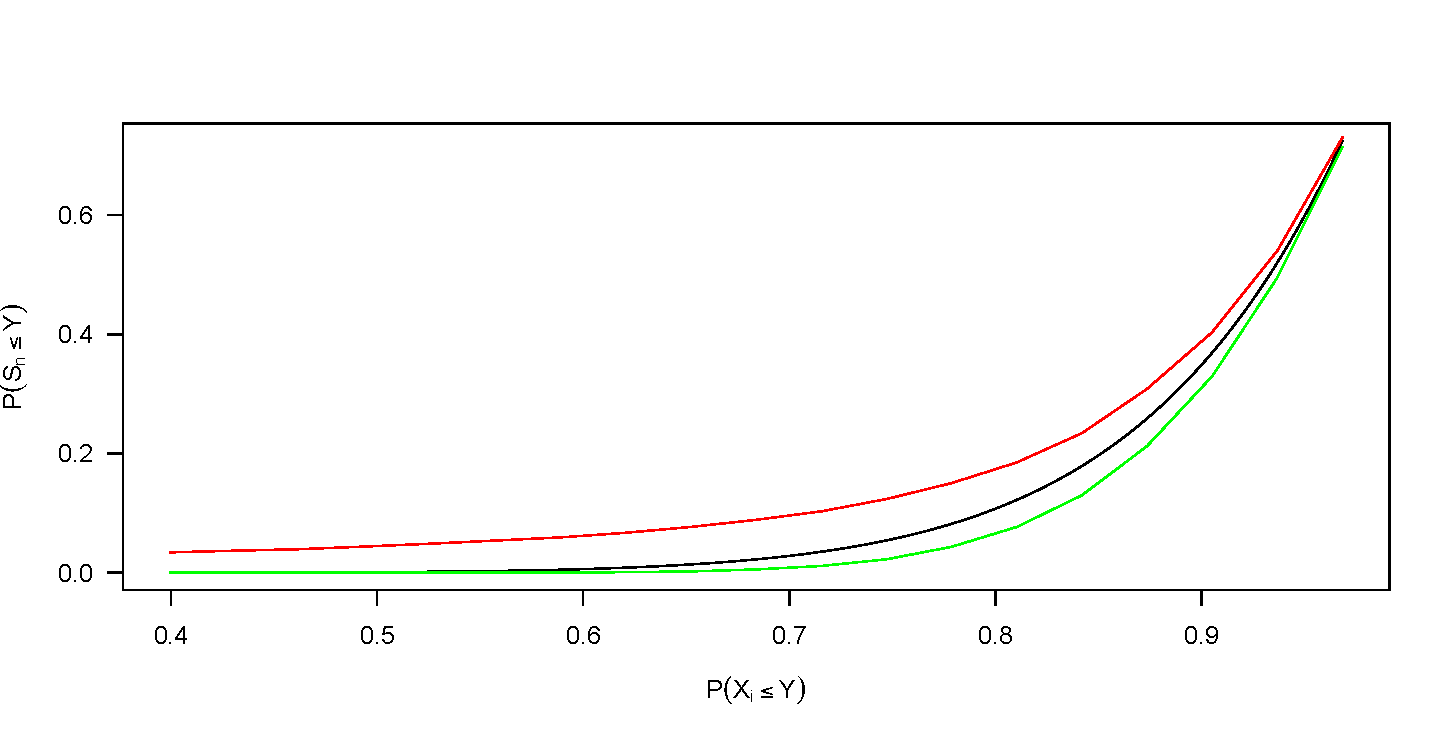
\includegraphics[width = 0.9\textwidth]{FunWithStatsPlot.pdf}}
\vspace{-.1 in}
\caption{Approximating $P(S_n \leq Y)$ with $\prod_{i = 1}^n P(X_i \leq Y)$ (black curve). The green curve represents a light-tailed random variable, with $P(Y \leq y) = 1 - e^{-y^2}$. The red curve represents a heavy-tailed random variable, with $P(Y \leq y) = 1 - (1+x)^{-1/\log(2)}$. It would be interesting to better understand the conditions under which the approximation is and isn't good.}
\label{fig:numerics}
\end{figure}

\newpage

\section{Code}

{\footnotesize
\begin{lstlisting}[language=R]
n = 10
N = 10^5

P = rep(1:19)/20
l = rep(0,length(P))
e = rep(0,length(P))
h = rep(0,length(P))
for(i in 1:19){
	p = P[i]
	k = 1 
	a = 1/log(2) 
	countL = 0
	countE = 0
	countP = 0
	for(j in 1:N){
		x = rbinom(1,n,p) #X_i is bernoulli with probability p
		U = runif(1)
		yL = sqrt(-log(U)) #Light Tailed; F(x) =  1- exp(-x^2)
		yE = -log(U) #Exponential; F(x) =  1- exp(-x)
		yP = U^(-1/a) - 1  #Power Law; F(x) = 1- (1+x)^{-a}
		if(x < yL) countL = countL+1
		if(x < yE) countE = countE+1
		if(x < yP) countP = countP+1
	}
	l[i] = countL/N
	e[i] = countE/N
	h[i] = countP/N
}
x = 1 - P + P*exp(-k)
plot(function(x){return(x^n)},xlim=c(min(x),max(x)),ylim=c(0,max(x)^n),ylab=expression(P(S[n] <= Y)),xlab=expression(P(X[i]<=Y)),las=1)
lines(x,l,col='green')
lines(x,e,col='blue')
lines(x,h,col='red')
\end{lstlisting}
}

%{\bf Note:} This was prompted by a question from Matt Weinberg, and caused me to stay up late at night, in a hotel room, with Charlotte.

%{\bf Possible Story:} You are a manager for a store. No customers are in the store, and you have a set of tasks to finish. What is the chance that you finish them all before the next customer walks in?

%\subsection{The Fact}
%%
%{\color{blue} Trying to make it seem surprising -- why are these quantities even related?
%Let $A_k$ be the event $\{X_k \leq Y\}$. Clearly $\{S_n \leq Y\} \subseteq A_k$ for each $k$, and therefore
%\[P(S_n \leq Y) \leq P( \cap_{i = 1}^n A_k)\]
%However, we also have 
%\[ \Pi_{i = 1}^k P(X_k \leq Y) \leq P( \cap_{i = 1}^n A_k),\]
%because the events $A_k$ are positively correlated.
%
%Magically, these two ``errors" cancel out perfectly when $Y$ is exponentially distributed!}


%\subsection{Proof}
%
%{\color{blue} More formal approach:
%
%For $k = 1, \ldots, n$, let $Z_k$ be the indicator that $S_k \leq Y$. %Then $Z_1 \geq Z_2 \geq \cdots \geq Z_n = {\bf 1}(X \leq Y)$.
%
%
%\begin{equation} P(Z_n = 1) = \Pi_{k = 1}^n P(Z_k = 1 \vert Z_{k-1} = 1)  \label{eq:decompose} \end{equation}
%
%We claim that 
%\begin{equation} P(Z_k = 1 \vert Z_{k-1} =1) = P(X_k \leq Y). \label{eq:memoryless}  \end{equation} 
%%\begin{equation} P(S_k \leq Y \vert S_{k-1} \leq Y) = P(X_k \leq Y). \end{equation} 
%
%By iterated expectation, 
%\[P(Z_k = 1 \vert Z_{k-1}) = E_{S_{k-1}}[P(Z_k = 1 \vert S_{k-1}, Z_{k-1})].\]
%But because $Y$ is memoryless, for every realization of $S_{k-1}$ and $Z_{k-1}$ we have 
%\[P(Z_k = 1 \vert S_{k-1}, Z_{k-1}) = Z_{k-1} P(S_{k-1} + X_k \leq Y \vert S_{k-1} \leq Y) = Z_{k-1}P(X_k \leq Y).\]
%}



%\subsection{Extensions: Non-exponential $Y$}

%Note that \eqref{eq:decompose} doesn't depend on the fact that $Y$ is exponential, but \eqref{eq:memoryless} does. 
%
% Suppose that for all $x \geq 0$, $P(Y - y \geq x \vert Y \geq y)$ is increasing/decreasing in $y$ ($Y$ is heavy/light tailed). Then we should get that $P(S_k \leq Y \vert S_{k-1} \leq Y)$ is larger/smaller than $P(X_k \leq Y)$, and therefore that $P(X \leq Y)$ is larger/smaller than the product. Code to test this out is in WeinbergStatsQ.R






\end{document}  